%\documentclass[crop,tikz,convert={outext=.svg,command=\unexpanded{pdf2svg \infile\space\outfile}},multi=false]{standalone}[2012/04/13]

\documentclass[tikz]{standalone}
\usetikzlibrary{arrows,shapes,fit,calc,positioning,intersections}
\makeatletter
\begin{document}
  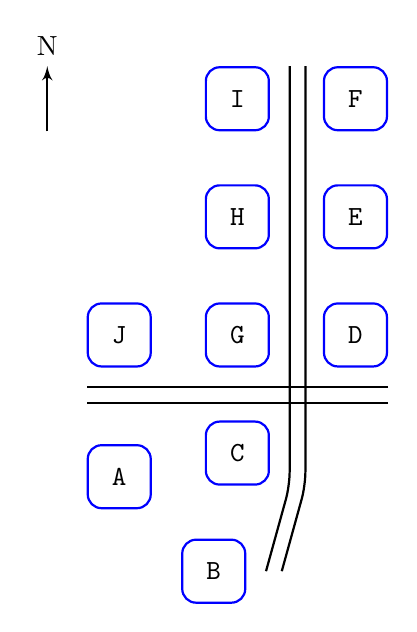
\begin{tikzpicture} [rounded corners=5pt,>=latex',thick]
    \tikzset {
      node distance=1.5cm,
      building/.style={rectangle,draw=blue,minimum width=0.8cm,minimum height=0.8cm}
    }
    \node [building] (i) {\ttfamily I};
    \node [building, below of=i] (h) {\ttfamily H};
    \node [building, below of=h] (g) {\ttfamily G};
    \node [building, below of=g] (c) {\ttfamily C};
    \node [building, right of=i] (f) {\ttfamily F};
    \node [building, below of=f] (e) {\ttfamily E};
    \node [building, below of=e] (d) {\ttfamily D};
    \node [building, left of=g] (j) {\ttfamily J};
    \node [building, left of=c, yshift=-0.3cm] (a) {\ttfamily A};
    \node [building, below of=c, xshift=-0.3cm] (b) {\ttfamily B};
    \draw [->] ([xshift=-2cm]i.south west) to ([xshift=-2cm]i.north west);
    \node [above] at ([xshift=-2cm]i.north west) {N};
    \draw ([xshift=0.25cm]i.north east) to ([xshift=0.25cm]c.south east) to ([xshift=0.25cm]b.east);
    \draw ([xshift=0.45cm]i.north east) to ([xshift=0.45cm]c.south east) to ([xshift=0.45cm]b.east);

    \draw ([yshift=-0.25cm]d.south east) to ([yshift=-0.25cm]j.south west);
    \draw ([yshift=-0.45cm]d.south east) to ([yshift=-0.45cm]j.south west);
  \end{tikzpicture}
\end{document}
